\chapter{Design}

\section{Authentication Policies}
Design of the Authentication policies, or as described in the specification as a Policy engine, provides the ability to comply with requirements specified by the administrator.
When users are trying to access the application, they need to meet certain conditions in order to achieve a successful login.
There may be some company or federal restrictions to particular services that need to be conformed to.

For instance, there might be some requirements to deny users access to the application from a specific country or specific types of devices.

It needs to be determined in which authentication process phases these policies should be evaluated.
Policies might be required to comply with some preconditions in order to be able to evaluate them.
It means that the environment context needs to be aligned with the policy requirement, such as gathering information about the user attempting to log in.

A particular hierarchy in policy priorities needs to be assessed as well in order to evaluate specific policies before others.
It provides the capability to create a more complex and comprehensive evaluation pipeline for authentication policies.

Every authentication policy consists of several conditions and actions.
All conditions must be met in order to execute specific actions.
If some of these conditions are not evaluated to be true, the whole authentication policy is skipped, and the following policy in the hierarchy structure is evaluated.

Authentication policies can be specified interactively via the administrator console or HTTP REST API.
All of them are stored in persistent storage, so every change of the structure is visible even after the re-initialization of the application. 
Specific operations can be executed on the policy entities, such as obtaining a specific authentication policy, creating a new one, or updating or removing the existing one.
Moreover, the priority to achieve the required hierarchy structure can be defined as well.

\subsection{Authentication Flow}

Authentication policies are tightly coupled to the authentication flows described in the section \ref{keycloak-authentication-flows}.
Authentication policies are a specific subset of authentication flows as these policies are basically just conditional authentication flows.

Conditional flows provide the majority of the required functionality to meet requirements for authentication policies or the policy engine.
It means that specific conditions are evaluated, and if all pass, specific actions are executed.

One of the major issues around authentication policies is manageability.
Administrators should not add a higher number of conditional flows to their existing authentication flows as these concepts should be separated in this manner.

Authentication policies extend the capabilities around the authentication flow process as they can be defined for the whole realm, not even for a specific flow.
To be more specific, it gives the possibility to share policies across different flows, which is the main difference between conditional flows and authentication policies.

It provides more fine-grained authentication policy management and a better authentication settings approach.

\subsection{Authentication Policy Authenticator}
In order to properly evaluate all authentication policies specified for the realm without the need to comprehensively expand the authentication flows, a specific authenticator was introduced.
It provides the ability to have a more fine-grained approach for these evaluations, as the administrator can specify in which phases of the authentication flow these policies will be processed.

The authenticator works as a configurable placeholder for these policies, as it can contain multiple configuration properties to asses the overall policies processing.
It might be possible to hide the authenticator from the flows completely, but the explicit settings provide a more deterministic approach.

The default authenticator configuration contains only a boolean flag to determine whether the user information is required for the evaluations or not.

When the authentication flow processing is in the phase of evaluating the authenticator, multiple steps are executed:

\begin{enumerate}
    \item \textbf{Obtain} -- Obtain all authentication policies.
    \item \textbf{Filter} -- Filter policies based on the authenticator configuration.
    \item \textbf{Process} -- Process all authentication policies.
    \item \textbf{Return} -- Return to the parent authentication flow and continue with processing other steps.
\end{enumerate}

When all conditions are met for an arbitrary policy, and the action explicitly allows access to the user, the authenticator itself is evaluated as successful without any other policy evaluations.

The same applies to the case when the action explicitly denies access to the user, the authenticator is evaluated as false, and the whole authentication flow processing is stopped.

Otherwise, when the action is not terminal, the other policies are evaluated as usual.

\subsection{Administrator Console}
// TODO add screenshots of admin pages and elaborate on them

\subsection{User Context condition}
// TODO explain user context in prior parent section and extend it here

\subsection{Policy Evaluation Example}
For a better representation of the authentication policy evaluation, a simple example with the described configuration might be considered.
The specification of a particular authentication policy is done through the administrator console in the Authentication section and Authentication Policies tab.

The following simple example of the authentication policy, in figure \ref{fig:design-policy-browser-flow}, has one condition and one action.
If the first condition is met, the underlying action is executed.

The policy contains a condition based on the current browser properties, which does not allow a specific browser vendor - Mozilla Firefox, in this case.
When the condition is met, access to the application is denied to the user.
This means that authentication requests can only be made via a browser other than Mozilla Firefox.

\begin{figure}[htbp]
  \centering
  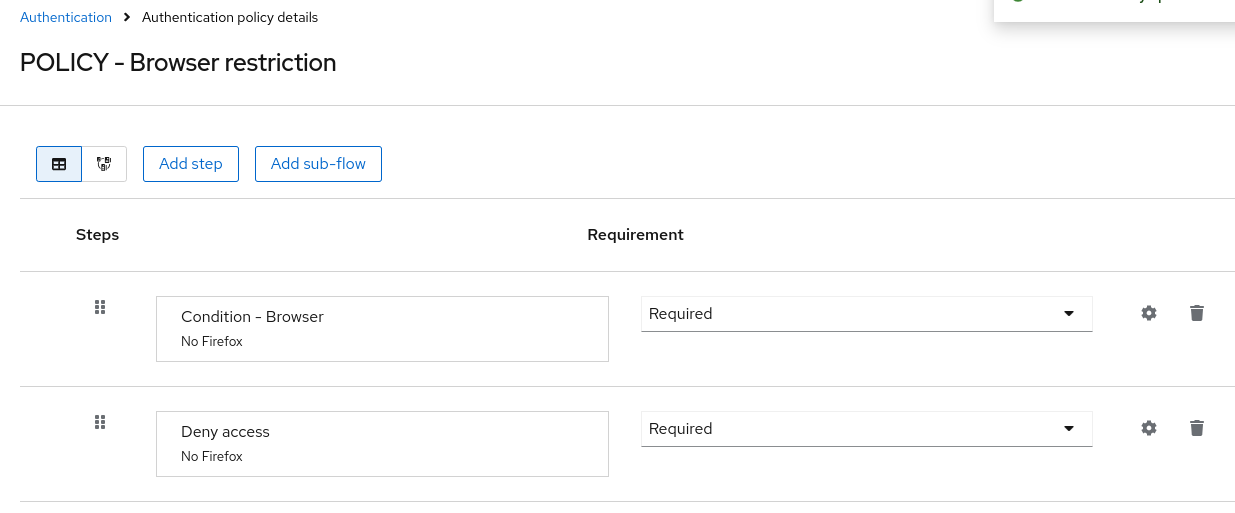
\includegraphics[width=1\textwidth]{img/sections/5-design/policy-browser-flow.png}
  \label{fig:design-policy-browser-flow}
  \caption{Authentication policy browser restriction}
\end{figure}

For a better visualization of the condition evaluation flow, consider this diagram:

\begin{figure}[htbp]
  \centering
  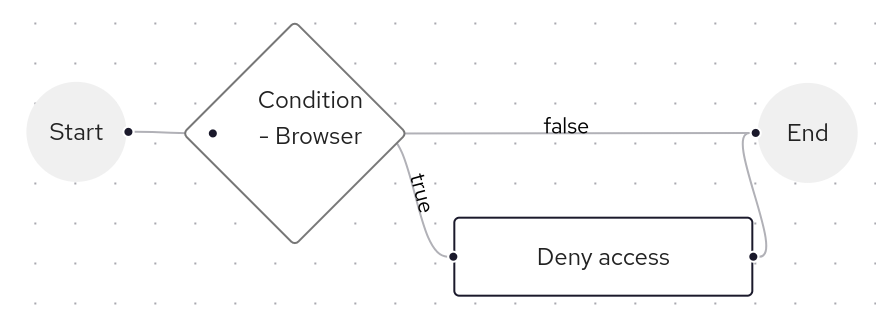
\includegraphics[width=0.8\textwidth]{img/sections/5-design/policy-browser-flow-graph.png}
  \label{fig:design-policy-browser-flow-graph}
  \caption{Authentication policy browser restriction graph}
\end{figure}

The condition configuration attributes differ based on the used condition provider/implementation.
Every condition provider specifies a set of configuration properties for condition settings.

The browser condition, shown in Figure \ref{fig:design-policy-browser-flow-condition}, includes \textit{Alias}, \textit{Operation}, and \textit{Browser} properties.
The \textit{Alias} is just a name for the condition, \textit{Operation} provides the possibility to choose one option from a list of operations, and \textit{Browser} is the direct value for the evaluations.

In this case, the condition is met only when the browser vendor is Firefox:

\begin{figure}[htbp]
  \centering
  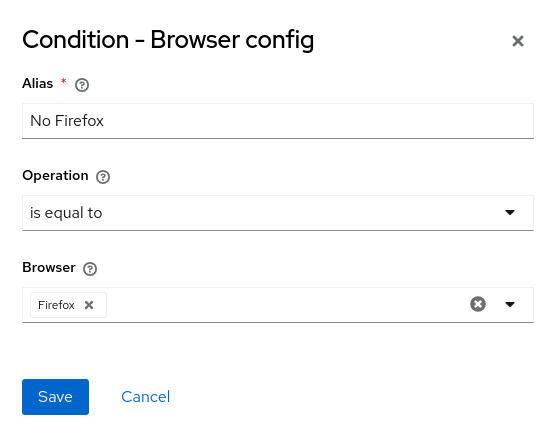
\includegraphics[width=0.8\textwidth]{img/sections/5-design/policy-browser-condition.png}
  \label{fig:design-policy-browser-flow-condition}
  \caption{Browser restriction condition}
\end{figure}

The action configuration also differs based on the provider of the action.
For the Deny access provider, visible in Figure \ref{fig:design-policy-browser-flow-deny}, the only additional property is \textit{Error Message}.
It represents an error message that is shown to the user when the access is denied.

\begin{figure}[htbp]
  \centering
  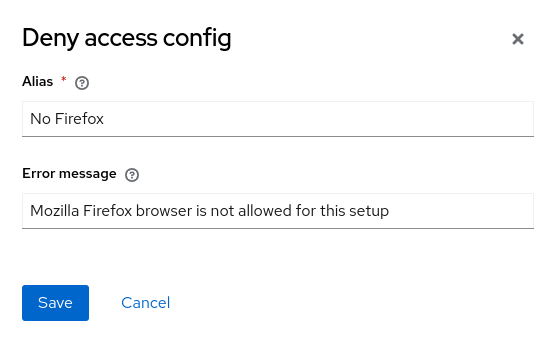
\includegraphics[width=0.8\textwidth]{img/sections/5-design/policy-browser-deny.png}
  \label{fig:design-policy-browser-flow-deny}
  \caption{Browser restriction deny access}
\end{figure}

\newpage
\section{Risk-based Authentication}
\subsection{Concept}
\subsection{User Context}
\subsection{Risk Evaluators}
\subsection{Risk Engine}
\subsection{Risk Levels}
\subsection{Risk Level conditions}


\section{Artificial Intelligence}


\section{External Integration}